\chapter{Graph Isomorphism, Subgraph Isomorphism}

Rishnak was eagerly looking for Ajur because he wanted to share with him a new concepts and found Ajur and Jura walking along the bank of a (presumably haunted) pond in the cemetery. Rishnak started this session with a small variant on what they had been discussing. A graph, whose vertices are labeled, is called a labeled graph and one without labels for vertices is called an unlabeled graph. Two labeled graphs are equivalent if they are identical. The labeled graphs in Figures \ref{8g1} and \ref{8g11} are equivalent. The graph in Figure \ref{8g2} is not equivalent to the graph in Figures \ref{8g1} or \ref{8g11} or as there is no edge between vertices 1 and 2.
\begin{figure}
\begin{center}
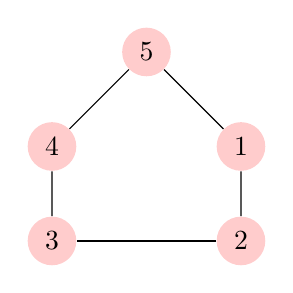
\begin{tikzpicture}
  [scale=.6,auto=left,every node/.style={circle,fill=red!20}]
  \node (n1) at (5,5) {1};
  \node (n4) at (1,5)  {4};
  \node (n3) at  (1,3) {3};
  \node (n2) at (5,3)  {2};
  \node (n5) at (3,7)  {5};

  \foreach \from/\to in {n1/n2,n2/n3,n3/n4,n4/n5,n1/n5}
    \draw (\from) -- (\to);

\end{tikzpicture}
\caption{Labeled Graph}\label{8g1}
\end{center}

\end{figure}
\begin{figure}
\begin{center}
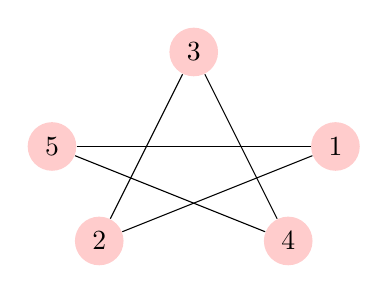
\begin{tikzpicture}
  [scale=.6,auto=left,every node/.style={circle,fill=red!20}]
   \node (n1) at (6,5) {1};
  \node (n5) at (0,5)  {5};
  \node (n2) at  (1,3) {2};
  \node (n4) at (5,3)  {4};
  \node (n3) at (3,7)  {3};

  \foreach \from/\to in {n1/n2,n2/n3,n3/n4,n4/n5,n5/n1}
    \draw (\from) -- (\to);

\end{tikzpicture}
\caption{ Another labeled graph with five vertices equivalent to Figure \ref{8g1}}\label{8g11}
\end{center}
\end{figure}

\begin{figure}
\begin{center}
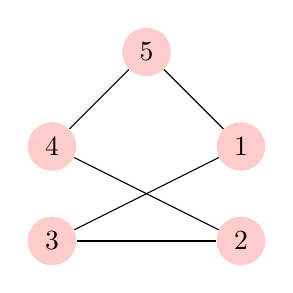
\begin{tikzpicture}
  [scale=.6,auto=left,every node/.style={circle,fill=red!20}]
   \node (n1) at (5,5) {1};
  \node (n4) at (1,5)  {4};
  \node (n3) at  (1,3) {3};
  \node (n2) at (5,3)  {2};
  \node (n5) at (3,7)  {5};


  \foreach \from/\to in {n1/n3,n2/n4,n3/n2,n1/n5,n5/n4}
    \draw (\from) -- (\to);

\end{tikzpicture}
\caption{ Another labeled graph with five vertices which is not equivalent to Graphs \ref{8g1} and \ref{8g11} as the edge labels are distinct from either of the two graphs}\label{8g2}
\end{center}
\end{figure}

Rishnak continued rhetorically: ``When are two graphs the same"? Two graphs are isomorphic (\emph{structurally the same}), if they are equivalent under a vertex relabeling. For example, if in the graph of Figure \ref{8g2} vertex 2 is relabeled as 3 and vertex 3 is relabeled as 2, then two graphs in Figures \ref{8g2} and \ref{8g1} are equivalent. If a graph, $G$, is equivalent to a graph $H$ and $H$ is equivalent to another graph $P$, then $G$ is equivalent to graph $P$\footnote{In other words, the relation of being equivalent graphs is transitive.}. To test whether two graphs are isomorphic are not is a hard problem\footnote{Not as hard as finding a Hamiltonian cycle in a graph} .

If two graphs are isomorphic, they should have the same number of vertices, the same number of edges, the same degree sequences, the same length of the longest cycle, and the same length of the shortest cycle.  These properties of graphs are called graph invariants. By no mean are these invariants are exhaustive. We do not know of a single easily computable invariant that can be used to test whether or not two given graphs are isomorphic. 

Rishnak asked Ajur, to provide two graphs which have the same number of vertices and same number of edges but they are not isomorphic. Ajur thought a bit and he was able to produce the following two graphs which have 6 vertices and 9 edges. Ajur added that one graph, Figure \ref{8g3}, is bipartite (all cycles are of even length)  and the other one, Figure \ref{8g4}, is not bipartite (it has cycle of length 3) and hence these two graphs are not isomorphic.

\begin{figure}

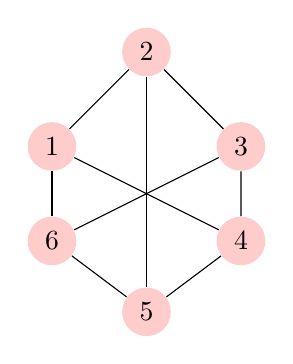
\begin{tikzpicture}
  [scale=.3,auto=left,every node/.style={circle,fill=red!20}]
  \node (n1) at (1,7) {1};
  \node (n2) at (5,11)  {2};
  \node (n3) at (9,7)  {3};
  \node (n4) at (9,3) {4};
  \node (n5) at (5,0)  {5};
  \node (n6) at (1,3) {6};
  
   \foreach \from/\to in {n1/n2,n2/n3,n3/n4,n4/n5,n5/n6,n1/n6,
  n2/n5, n6/n3,n1/n4}
    \draw (\from) -- (\to);
    \end{tikzpicture}
\caption{ A Bipartite Graph with 6 vertices and 9 edges same as graph in \ref{5g5}}\label{8g3}

\end{figure}

\begin{figure}

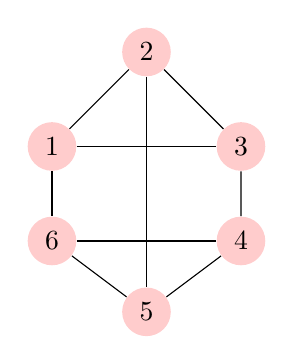
\begin{tikzpicture}
  [scale=.3,auto=left,every node/.style={circle,fill=red!20}]
  \node (n1) at (1,7) {1};
  \node (n2) at (5,11)  {2};
  \node (n3) at (9,7)  {3};
  \node (n4) at (9,3) {4};
  \node (n5) at (5,0)  {5};
  \node (n6) at (1,3) {6};
  
   \foreach \from/\to in {n1/n2,n2/n3,n3/n4,n4/n5,n5/n6,n1/n6,
  n2/n5, n6/n4,n1/n3}
    \draw (\from) -- (\to);
    \end{tikzpicture}
\caption{ A non-bipartite graph with 6 vertices and 9 edges}\label{8g4}

\end{figure}

Ajur thought for a while and said that partial solutions to the isomorphism problem would be very useful when you want to test whether a given graph is in a collection of graphs, a problem that comes up in chemistry. Rishnak was pleased to notice that Ajur was thinking about practical applications of graph theory. 

Ajur wanted to know if there is an easier method for testing isomorphism between rooted trees. Rishnak smiled and said there is a faster method for rooted trees. First, Rishnak explained a certain canonical representation for a labeled tree, called a Pr\"ufer code. The construction is iterative, and the Pr\"ufer code of a labeled tree with $n$ vertices is a code of length $n-2$. First, we recall that a leaf of a tree is a vertex that is connected to only one other vertex.

\begin{enumerate}
\item Let Pr{\"u}fer code be an empty.

\item Start with a leaf vertex of smallest label, say v. Find the vertex connecting it to the rest of tree say w.  Remove v from the tree and add w to the Pr{\"u}fer code.
 
\item Repeat the previous step until we are left with two vertices.
\end{enumerate}

We execute this procedure for the tree in Example \ref{8g5}. The smallest leaf vertex is 4. Its adjacent vertex is labeled 2. So 2 is added to the Pr{\"u}fer code and vertex 4 is removed. Next smallest vertex is 5 and its adjacent vertex is 2. Hence 2 is added to the Pr{\"u}fer code and vertex labeled 5 is removed. Now 2 is the smallest leaf vertex and its adjacent vertex is 1 and  1 is added to Pr{\"u}fer code and vertex 2 is removed. Currently Pr{\"u}fer code is \textbf{221}. Now 1 is the smallest labeled vertex and its adjacent vertex is 3 and vertex 1 is removed. Hence 3 is added to Pr{\"u}fer code which becomes \textbf{2213}. The next smallest leaf vertex is 6 and its adjacent vertex is 3. 3 is added to Pr{\"u}fer code. There are only two vertices left and we are done. The Pr{\"u}fer code for tree in Example \ref{8g5} is \textbf{22133}. From this Pr{\"u}fer code, one can conclude that there are 7 vertices in the tree (as the Pr{\"u}fer code is of length $n-2$ for a tree with $n$ vertices). Further, we can also conclude that vertices labeled 4,5,6 and 7 are leaf vertices as they do not appear in the given Pr{\'u}fer code. 
\begin{figure}
\begin{center}

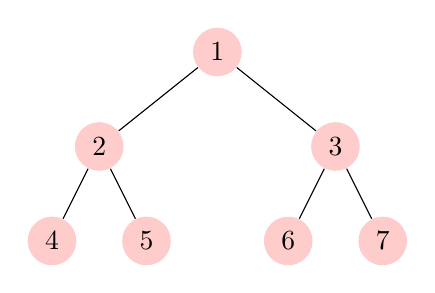
\begin{tikzpicture}
  [scale=.6,auto=left,every node/.style={circle,fill=red!20}]
  \node (n1) at (5.5,7) {1};
  \node (n2) at (3,5)  {2};
  \node (n3) at (8,5)  {3};
  \node (n4) at (2,3) {4};
  \node (n5) at (4,3)  {5};
  \node (n6) at (7,3)  {6};
  \node (n7) at (9,3)  {7};

  \foreach \from/\to in {n1/n2,n1/n3,n2/n4,n2/n5,n3/n6,n3/n7}
    \draw (\from) -- (\to);

\end{tikzpicture}

\caption{Tree with 7 vertices and four leaf vertices }\label{8g5}
\end{center}
\end{figure}

Ajur then wanted to know if one could have a code for unlabeled trees. Rishnak replied with a resounding yes and explained the basic steps for a rooted tree. For any tree, one needs to choose an appropriate root vertex: \footnote{Center of a tree is chosen as the root vertex}  %\textbf{Raju: be careful, not every tree has a center which is a vertex!}} 
\begin{enumerate}
    \item  Label the leaf vertices as 01;
    \item Let $x$ be a non-leaf vertex. If all the children of $x$, sort these labels in alphabetical order. \footnote{0 comes before 1} The label of vertex $x$ is 0 followed by concatenation of the (sorted) labels of the children followed by 1;
    \item Stop after you label the root vertex.
\end{enumerate}

For example for the tree in \ref{8g5} leaf vertices 4,5,6,7 are all labeled \textbf{01}. Vertex 2 is labeled \textbf{001011} and vertex 3 has a similar label \textbf{001011}. Finally root vertex has the label \textbf{00101100101111}. This \textbf{00101100101111} becomes the code for the tree.

Rishnak continued that closely related to Graph Isomorphism is a problem that has plenty of uses in real life - and not just in the ghoulish realm. Ajur chuckled at the bad joke but politely retrained from interrupting. Rishnak continued with the statement of the next problem.  Instead of asking whether two graphs are structurally similar, given two graphs $G$ and $H$, the subgraph isomorphism problem is if there is a sub-graph of $G$ that is isomorphic to H. Ajur responded immediately saying this approach can be used to test if a graph $G$ with $n$ vertices has a Hamiltonian cycle by choosing $H$ to be a cycle of length $n$ and asking whether there is a sub-graph of $G$ isomorphic to $H$. Rishnak nodded in agreement and said that is the reason the sub-graph Isomorphism problem is hard. On the other hand, if both $G$ and $H$ are labeled graphs, there are heuristics to test whether $H$ occurs in $G$ as a sub-graph. This type of labeled sub-graph isomorphism problem has many applications in medical imaging and chemical structure identifications.

\textbf{Question for the sixth day:} Draw a tree whose Pr{\"u}fer code is 232.

\textbf{Answer} Ajur realized that this is a tree with five vertices and he drew the following tree in Figure \ref{6q1}.
\begin{figure}
\begin{center}

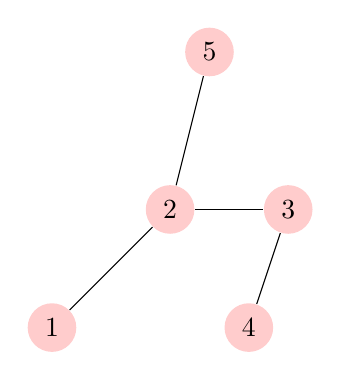
\begin{tikzpicture}
  [scale=.5,auto=left,every node/.style={circle,fill=red!20}]
  \node (n1) at (0,0) {1};
  \node (n2) at (3,3)  {2};
  \node (n3) at (6,3)  {3};
  \node (n4) at (5,0) {4};
  \node (n5) at (4,7)  {5};
 

  \foreach \from/\to in {n1/n2,n4/n3,n2/n3,n2/n5}
    \draw (\from) -- (\to);

\end{tikzpicture}

\caption{Tree with 5 vertices}\label{6q1}
\end{center}
\end{figure}

Rishnak was happy with Ajur's answer and Ajur was eager to go with Jura.